% !TEX encoding = UTF-8 Unicode
\level{2}{Fase CP: Completion of the Product}
	\textbf{Periodo}: dal \insdate{03}{05}{2015} al \insdate{24}{05}{2015} \\Questa fase comincia subito dopo la consegna per la \insphase{Fase IP} e termina con l'incontro con il proponente per mostrare il prototipo con tutti i requisiti implementati e con la scadenza della consegna per la \insrev{Revisione di Qualifica}. 
	\\Le attività di questa fase saranno le seguenti:
	\begin{itemize}
		\item\textbf{Definizione di Prodotto}: viene steso il documento \insdoc{Definizione di Prodotto v3.00}. Esso definisce la struttura interna del sistema e le relazioni dei componenti del prodotto relativi ai requisiti obbligatori, desiderabili ed opzionali.
		\item \textbf{Codifica}: con quest'attività inizia lo sviluppo da parte dei programmatori dei requisiti opzionali. Sarà dunque seguito quanto riportato nel documento \insdoc{Definizione di Prodotto v3.00};
		\item \textbf{Esecuzione test}: verranno eseguiti automaticamente tutti i test di unità e di integrazione previsti dal documento \insdoc{Piano di Qualifica v6.00};
		\item\textbf{Manuale Utente e Manuale Amministratore}: vengono ampliati ed aggiornati i manuali che forniranno indicazioni agli utilizzatori del sistema.
		\item\textbf{Incremento e Verifica Documenti}: vengono eseguite modifiche ai documenti già scritti, se necessario, che passeranno alla versione 6.00.
		\item\textbf{Glossario}: vengono aggiunti al file \insfile{Glossario.xml} i vocaboli dei quali si ritiene necessaria una definizione formale. Alla fine di questa fase viene quindi generato il documento \insdoc{Glossario v6.00}.
	\end{itemize}
	\level{3}{Diagramma di Gantt delle attività}
	\begin{figure}[H]\centering
		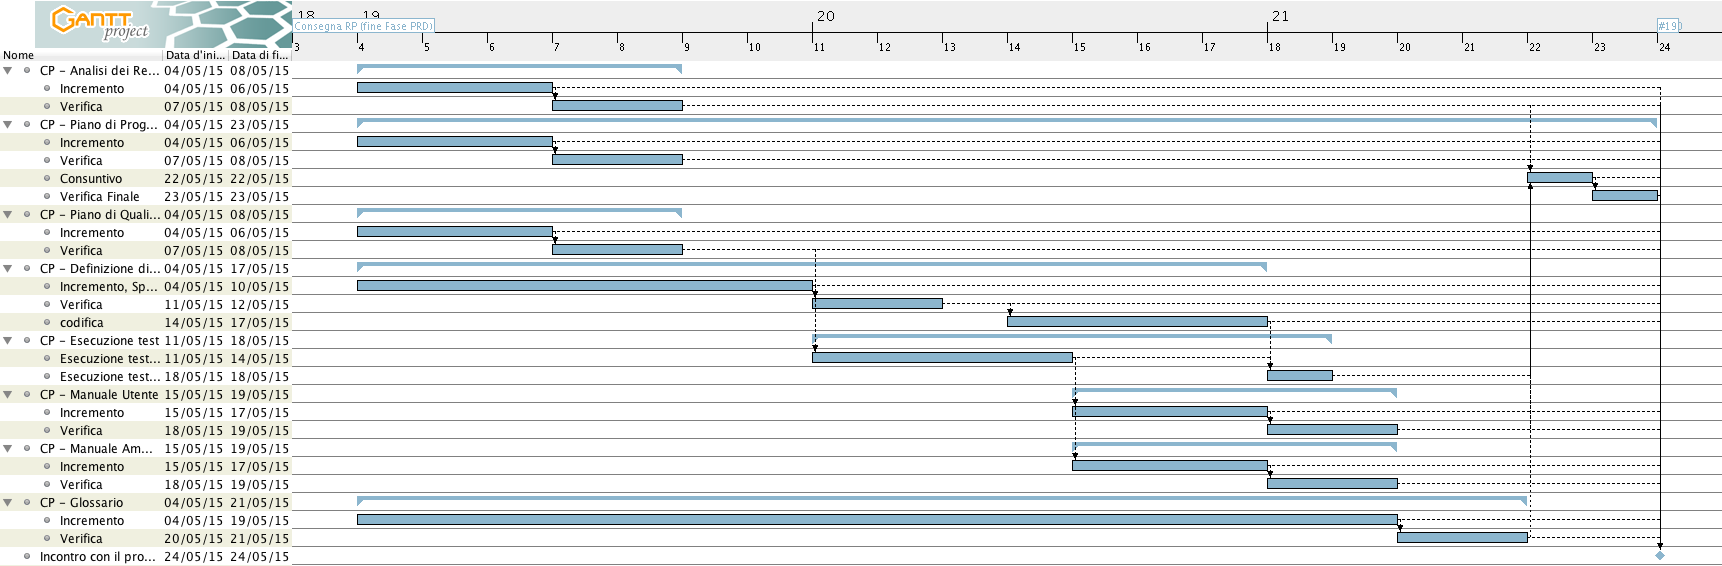
\includegraphics[width=\textwidth]{PianoDiProgetto/Pics/FaseCP.png}
	\caption{Gantt Fase CP}
\end{figure}
